\documentclass[aspectratio=169,12pt]{beamer}
\usepackage[utf8]{inputenc}
\usepackage{amsmath, amssymb}
\usepackage{booktabs}
\usepackage{colortbl}
\usepackage{hyperref}
\usepackage{makecell}
\usepackage{ragged2e}
\usepackage{tikz}
\usetikzlibrary{arrows.meta, positioning, shapes.geometric, calc, tikzmark, shapes.misc, fit, decorations.pathreplacing, matrix, shapes.callouts}
\usepackage{tcolorbox}
\usepackage{array}
\usepackage{listings}
\usepackage{pgfkeys}
\usepackage{adjustbox}
\usepackage[normalem]{ulem}
\usepackage{arydshln} 
\usetheme{Madrid}

% Custom colors - consolidated
\definecolor{correctgreen}{RGB}{0,150,0}
\definecolor{incorrectred}{RGB}{200,0,0}
\definecolor{counterblue}{RGB}{70,130,255}
\definecolor{highlightyellow}{RGB}{255,230,100}
\definecolor{lightblue}{RGB}{240,248,255}
\definecolor{darkblue}{RGB}{0,100,200}
\definecolor{highlightorange}{RGB}{255,200,100}

% Stage description box style (no title)
\tcbset{
    stagebox/.style={
        colback=red!5!white,
        colframe=red!75!black,
        boxrule=0.5pt,
        arc=2pt,
        left=4pt,
        right=4pt,
        top=4pt,
        bottom=4pt,
        fontupper=\small
    }
}

% PGF Keys for pipeline diagram configuration
\pgfkeys{
    /pipeline/.cd,
    % Stage colors
    ifcolor/.initial=lightblue,
    idcolor/.initial=lightblue,
    excolor/.initial=lightblue,
    memcolor/.initial=lightblue,
    wbcolor/.initial=lightblue,
    % Stage contents (instruction labels)
    ifcontent/.initial={},
    idcontent/.initial={},
    integercontent/.initial={},
    multiplycontent/.initial={},
    dividercontent/.initial={},
    memcontent/.initial={},
    wbcontent/.initial={},
    % Instruction list
    instructions/.initial={},
    % Highlight colors for specific units
    highlightinteger/.initial=white,
    highlightmultiply/.initial=white,
    highlightdivider/.initial=white,
    % Individual multiply stage highlights
    highlightM1/.initial=white,
    highlightM2/.initial=white,
    highlightM3/.initial=white,
    highlightM4/.initial=white,
    % Individual divider stage highlights
    highlightD1/.initial=white,
    highlightD2/.initial=white,
    highlightD3/.initial=white,
    highlightD4/.initial=white,
    highlightD5/.initial=white,
    highlightD6/.initial=white,
    % Y-spacing between execution unit rows (EX, M, D)
    yspacing/.initial=1.2cm,
    % Show callouts describing units (for first appearance)
    showcallouts/.initial=false,
    % Add extra 3mm spacing between rows
    spaced/.initial=false,
    % Which M stage (1-4) to position multiply label above
    multiplystage/.initial=0,
    % Individual instructions (for colored display)
    inst1/.initial={},
    inst2/.initial={},
    inst3/.initial={},
    % Checkmarks for completed instructions (true/false)
    inst1done/.initial=false,
    inst2done/.initial=false,
    inst3done/.initial=false
}

% TikZ styles for pipeline diagram
\tikzset{
    pipeline stage/.style={draw=darkblue!50, fill=lightblue, minimum width=1.2cm, minimum height=0.8cm},
    exec unit/.style={draw, minimum width=0.8cm, minimum height=0.6cm},
    exec unit small/.style={draw, minimum width=0.6cm, minimum height=0.6cm},
    code box/.style={draw, thick, rounded corners=2pt, inner sep=4pt, align=left, font=\footnotesize},
    unit callout/.style={
        rectangle callout,
        draw,
        fill=yellow!20,
        font=\footnotesize,
        inner sep=3pt,
        callout absolute pointer={#1}
    },
}

% Macro for drawing the pipeline diagram
\newcommand{\drawPipeline}[1][]{%
    \pgfkeys{/pipeline/.cd,#1}%
    % Calculate extra spacing (add 3mm if spaced=true)
    \pgfkeysgetvalue{/pipeline/spaced}{\pipelinespaced}
    \def\spacedtrue{true}
    \ifx\pipelinespaced\spacedtrue
        \def\extraspacing{0.3cm}
    \else
        \def\extraspacing{0cm}
    \fi
    \begin{tikzpicture}[scale=0.8, transform shape]
        % Pipeline stages IF and ID
        \node[pipeline stage, fill=\pgfkeysvalueof{/pipeline/ifcolor}] (IF) {IF};
        \node[pipeline stage, fill=\pgfkeysvalueof{/pipeline/idcolor}, right=of IF] (ID) {ID};

        % Multiply pipeline matrix (reference row)
        \matrix (mulmatrix) [
            matrix of nodes,
            right=2cm of ID.east,
            anchor=west,
            column sep=0.5cm,
            nodes={exec unit},
            ampersand replacement=\&,
        ] {
            |[fill=\pgfkeysvalueof{/pipeline/highlightM1}]| M1 \&
            |[fill=\pgfkeysvalueof{/pipeline/highlightM2}]| M2 \&
            |[fill=\pgfkeysvalueof{/pipeline/highlightM3}]| M3 \&
            |[fill=\pgfkeysvalueof{/pipeline/highlightM4}]| M4 \\
        };

        % Integer unit - centered above multiply row
        \node[exec unit, minimum width=1cm, fill=\pgfkeysvalueof{/pipeline/highlightinteger}]
            (EX) at ($(mulmatrix-1-2)!0.5!(mulmatrix-1-3) + (0,\pgfkeysvalueof{/pipeline/yspacing}+\extraspacing)$) {EX};

        % Divider pipeline matrix - centered below multiply row
        \matrix (divmatrix) [
            matrix of nodes,
            column sep=0.4cm,
            nodes={exec unit small},
            ampersand replacement=\&,
        ] at ($(mulmatrix-1-2)!0.5!(mulmatrix-1-3) + (0,-\pgfkeysvalueof{/pipeline/yspacing}-\extraspacing)$) {
            |[fill=\pgfkeysvalueof{/pipeline/highlightD1}]| D1 \&
            |[fill=\pgfkeysvalueof{/pipeline/highlightD2}]| D2 \&
            |[fill=\pgfkeysvalueof{/pipeline/highlightD3}]| D3 \&
            |[fill=\pgfkeysvalueof{/pipeline/highlightD4}]| D4 \&
            |[fill=\pgfkeysvalueof{/pipeline/highlightD5}]| D5 \&
            |[fill=\pgfkeysvalueof{/pipeline/highlightD6}]| D6 \\
        };

        % Execution label node (for fitting)
        \node[anchor=south west, yshift=4mm, font=\small] (execlabel) at (EX.north -| divmatrix-1-1.west) {Execution};

        % Execution box (includes label in fit)
        \node[draw, thick, dashed, fit=(EX)(mulmatrix)(divmatrix)(execlabel), inner sep=0.3cm] (execbox) {};

        % MEM and WB stages
        \node[pipeline stage, fill=\pgfkeysvalueof{/pipeline/memcolor}, right=3cm of mulmatrix-1-4.west] (MEM) {MEM};
        \node[pipeline stage, fill=\pgfkeysvalueof{/pipeline/wbcolor}, right=of MEM] (WB) {WB};

        % Connections from IF to ID
        \draw[->, thick] (IF) -- (ID);

        % Connections from ID to execution units
        \draw[->, thick] (ID.east) -- ([xshift=-2cm]EX.west) |- (EX.west);
        \draw[->, thick] (ID.east) -- (mulmatrix-1-1.west);
        \draw[->, thick] (ID.east) -- ([xshift=-3mm]divmatrix-1-1.west) -- (divmatrix-1-1.west);

        % Connections within multiply pipeline
        \draw[->, thick] (mulmatrix-1-1) -- (mulmatrix-1-2);
        \draw[->, thick] (mulmatrix-1-2) -- (mulmatrix-1-3);
        \draw[->, thick] (mulmatrix-1-3) -- (mulmatrix-1-4);

        % Connections within divider pipeline
        \draw[->, thick] (divmatrix-1-1) -- (divmatrix-1-2);
        \draw[->, thick] (divmatrix-1-2) -- (divmatrix-1-3);
        \draw[->, thick] (divmatrix-1-3) -- (divmatrix-1-4);
        \draw[->, thick] (divmatrix-1-4) -- (divmatrix-1-5);
        \draw[->, thick] (divmatrix-1-5) -- (divmatrix-1-6);

        % Connections from execution units to MEM
        \draw[->, thick] (EX.east) -- ([xshift=2cm]EX.east) -- ([xshift=-3mm]MEM.west) -- (MEM.west);
        \draw[->, thick] (mulmatrix-1-4.east) -- (MEM.west);
        \draw[->, thick] (divmatrix-1-6.east) -- ([xshift=-3mm]MEM.west) -- (MEM.west);

        % Connection from MEM to WB
        \draw[->, thick] (MEM) -- (WB);

        % Add content labels to stages if specified
        \pgfkeysgetvalue{/pipeline/ifcontent}{\ifcontentval}
        \ifx\ifcontentval\empty\else
            \node[above=0.1cm of IF, font=\footnotesize, text=blue] {\ifcontentval};
        \fi

        \pgfkeysgetvalue{/pipeline/idcontent}{\idcontentval}
        \ifx\idcontentval\empty\else
            \node[above=0.1cm of ID, font=\footnotesize, text=blue] {\idcontentval};
        \fi

        \pgfkeysgetvalue{/pipeline/integercontent}{\intcontent}
        \ifx\intcontent\empty\else
            \node[above=0.1cm of EX, font=\footnotesize, text=blue] {\intcontent};
        \fi

        \pgfkeysgetvalue{/pipeline/multiplycontent}{\mulcontent}
        \ifx\mulcontent\empty\else
            % Position based on multiplystage parameter (0=default, 1-4=specific stage)
            \pgfkeysgetvalue{/pipeline/multiplystage}{\mulstage}
            \ifnum\mulstage=1
                \node[above=0.1cm of mulmatrix-1-1, font=\footnotesize, text=blue] {\mulcontent};
            \else\ifnum\mulstage=2
                \node[above=0.1cm of mulmatrix-1-2, font=\footnotesize, text=blue] {\mulcontent};
            \else\ifnum\mulstage=3
                \node[above=0.1cm of mulmatrix-1-3, font=\footnotesize, text=blue] {\mulcontent};
            \else\ifnum\mulstage=4
                \node[above=0.1cm of mulmatrix-1-4, font=\footnotesize, text=blue] {\mulcontent};
            \else
                \node[above=0.1cm of mulmatrix-1-2, font=\footnotesize, text=blue] {\mulcontent};
            \fi\fi\fi\fi
        \fi

        \pgfkeysgetvalue{/pipeline/dividercontent}{\divcontent}
        \ifx\divcontent\empty\else
            \node[above=0.1cm of divmatrix-1-3, font=\footnotesize, text=blue] {\divcontent};
        \fi

        \pgfkeysgetvalue{/pipeline/memcontent}{\memcontentval}
        \ifx\memcontentval\empty\else
            \node[above=0.1cm of MEM, font=\footnotesize, text=blue] {\memcontentval};
        \fi

        \pgfkeysgetvalue{/pipeline/wbcontent}{\wbcontentval}
        \ifx\wbcontentval\empty\else
            \node[above=0.1cm of WB, font=\footnotesize, text=blue] {\wbcontentval};
        \fi

        % Instruction list in a box (positioned above WB)
        % Check if individual instructions are provided (for highlighted display)
        \pgfkeysgetvalue{/pipeline/inst1}{\instOne}
        \pgfkeysgetvalue{/pipeline/inst2}{\instTwo}
        \pgfkeysgetvalue{/pipeline/inst3}{\instThree}
        \ifx\instOne\empty
            % Fall back to legacy instructions parameter
            \pgfkeysgetvalue{/pipeline/instructions}{\instlist}
            \ifx\instlist\empty\else
                \node[code box, above=0.8cm of WB] {\instlist};
            \fi
        \else
            % Get completion status for checkmarks
            \pgfkeysgetvalue{/pipeline/inst1done}{\instOneDone}
            \pgfkeysgetvalue{/pipeline/inst2done}{\instTwoDone}
            \pgfkeysgetvalue{/pipeline/inst3done}{\instThreeDone}
            \def\donetrue{true}
            % Use individual instructions with fixed colors (yellow, orange, cyan)
            \node[code box, above=0.8cm of WB, align=left] {%
                \colorbox{highlightyellow}{\instOne}\ifx\instOneDone\donetrue\,\textcolor{correctgreen}{\checkmark}\fi%
                \ifx\instTwo\empty\else\\[-0.5ex]\colorbox{highlightorange}{\instTwo}\ifx\instTwoDone\donetrue\,\textcolor{correctgreen}{\checkmark}\fi\fi%
                \ifx\instThree\empty\else\\[-0.5ex]\colorbox{cyan!40}{\instThree}\ifx\instThreeDone\donetrue\,\textcolor{correctgreen}{\checkmark}\fi\fi%
            };
        \fi

        % Callouts for first appearance (shown on click)
        \pgfkeysgetvalue{/pipeline/showcallouts}{\showcallouts}
        \def\calloutstrue{true}
        \ifx\showcallouts\calloutstrue
            \node<2->[unit callout={(EX.north)}, above left=0.3cm and 0.5cm of EX]
                {Integer ALU (1 cycle)};
            \node<2->[unit callout={(mulmatrix-1-1.north west)}, above left=0.3cm and 0.3cm of mulmatrix-1-1]
                {Multiply unit (4 cycles)};
            \node<2->[unit callout={(divmatrix-1-1.north west)}, above left=0.3cm and 0.3cm of divmatrix-1-1]
                {Divider unit (6 cycles)};
        \fi
    \end{tikzpicture}%
}

% Macro for ROB diagram
\newcommand{\drawROB}[1]{%
    \begin{tikzpicture}[baseline=(current bounding box.north)]
        \matrix (rob) [matrix of nodes,
            nodes={draw, minimum width=1.5cm, minimum height=0.45cm, anchor=center, font=\scriptsize},
            row sep=-\pgflinewidth,
            column sep=-\pgflinewidth,
            inner sep=0pt,
            label={above:\textbf{ROB}},
            ampersand replacement=\&
            ] {
            #1
        };
        \draw[decorate, decoration={brace, amplitude=5pt, mirror}, thick]
            ([xshift=0.3cm]rob.south east) -- ([xshift=0.3cm]rob.north east)
            node[midway, right=5pt, font=\small] {Cyclic Buffer};
    \end{tikzpicture}
}

% Commands for highlighting entries in detailed OOO diagrams
\newcommand{\oldentry}[1]{~#1}
\newcommand{\newentrya}[1]{\colorbox{highlightyellow}{#1}}
\newcommand{\newentryb}[1]{\colorbox{highlightorange}{#1}}
\newcommand{\newentryc}[1]{\colorbox{cyan!40}{#1}}
\newcommand{\srcentrya}[1]{\colorbox{highlightyellow!30}{#1}}
\newcommand{\srcentryb}[1]{\colorbox{highlightorange!30}{#1}}
\newcommand{\srcentryc}[1]{\colorbox{cyan!15}{#1}}

% PGF Keys for detailed OOO diagram configuration
\pgfkeys{
    /OOO/.is family, /OOO,
    default/.style = {
        % RAT registers
        R1 = {}, R2 = {}, R3 = {}, R4 = {},
        % ROB cells (2 columns x 5 rows: instruction with renamed regs, status OK/INV)
        rob01 = {}, rob02 = {},
        rob11 = {}, rob12 = {},
        rob21 = {}, rob22 = {},
        rob31 = {}, rob32 = {},
        rob41 = {}, rob42 = {},
        % RS cells
        rs1 = {~}, rs2 = {~}, rs3 = {~},
        % MOB cell
        mob1 = {~},
        % Execute cells
        exec1 = {}, exec2 = {},
        % Retire cells
        ret1 = {}, ret2 = {}, ret3 = {},
        % Instruction queue (5 rows)
        instq1 = {~}, instq2 = {~}, instq3 = {~}, instq4 = {~}, instq5 = {~}
    },
    % RAT mappings
    R1/.estore in = \prfOne,
    R2/.estore in = \prfTwo,
    R3/.estore in = \prfThree,
    R4/.estore in = \prfFour,
    % ROB cell contents
    rob01/.estore in = \robZeroOne, rob02/.estore in = \robZeroTwo,
    rob11/.estore in = \robOneOne, rob12/.estore in = \robOneTwo,
    rob21/.estore in = \robTwoOne, rob22/.estore in = \robTwoTwo,
    rob31/.estore in = \robThreeOne, rob32/.estore in = \robThreeTwo,
    rob41/.estore in = \robFourOne, rob42/.estore in = \robFourTwo,
    % RS cell contents
    rs1/.estore in = \rsOne,
    rs2/.estore in = \rsTwo,
    rs3/.estore in = \rsThree,
    % MOB cell contents
    mob1/.estore in = \mobOne,
    % Execute cell contents
    exec1/.estore in = \execOne,
    exec2/.estore in = \execTwo,
    % Retire cell contents
    ret1/.estore in = \retOne,
    ret2/.estore in = \retTwo,
    ret3/.estore in = \retThree,
    % Instruction queue (5 rows)
    instq1/.estore in = \instQOne,
    instq2/.estore in = \instQTwo,
    instq3/.estore in = \instQThree,
    instq4/.estore in = \instQFour,
    instq5/.estore in = \instQFive,
}

% Macro for drawing detailed OOO execution diagram
\newcommand{\OOODiagram}[1][]{%
    % Set defaults and process keys
    \pgfkeys{/OOO,default,#1}%
    %
    \begin{tikzpicture}[
        cell/.style={draw, minimum width=0.8cm, minimum height=0.35cm},
        smallcell/.style={draw, minimum width=0.6cm, minimum height=0.35cm},
        roundbox/.style={draw, ellipse, minimum width=3cm, minimum height=1.5cm},
        dashedbox/.style={draw, dashed, rectangle, minimum width=3cm, minimum height=1cm}
    ]
    %
    % RAT (Register Alias Table)
    \matrix[matrix of nodes,
            nodes={cell, anchor=center,
            minimum height=4mm,
            text height=1ex,
            text depth=0.25ex},
            column sep=-\pgflinewidth,
            row sep=-\pgflinewidth,
            inner sep=0pt,
            label={left:\textbf{RAT}},
            ampersand replacement=\&] (rat) {
        \scriptsize R1 \& \scriptsize \prfOne \\
        \scriptsize R2 \& \scriptsize \prfTwo \\
        \scriptsize R3 \& \scriptsize \prfThree \\
        \scriptsize R4 \& \scriptsize \prfFour \\
    };
    %
    % ROB (Reorder Buffer) - 3 columns (label, instruction with renamed regs, status)
    \matrix[matrix of nodes,
            column sep=-\pgflinewidth,
            row sep=-\pgflinewidth,
            inner sep=0pt,
            label={left:\textbf{ROB}},
            below=0.2cm of rat,
            anchor=north,
            nodes in empty cells,
            nodes={cell, align=left},
            column 1/.append style={nodes={text width=0.5cm, minimum height=4mm, text height=1ex, text depth=0.25ex}},
            column 2/.append style={nodes={text width=3.2cm, minimum height=4mm, text height=1ex, text depth=0.25ex}},
            column 3/.append style={nodes={text width=0.6cm, minimum height=4mm, text height=1ex, text depth=0.25ex}},
            ampersand replacement=\&
        ] (rob) {
    |[cell]| \scriptsize RB0 \& |[cell]| \scriptsize \robZeroOne  \& |[cell]| \scriptsize \robZeroTwo \\
    |[cell]| \scriptsize RB1 \& |[cell]| \scriptsize \robOneOne   \& |[cell]| \scriptsize \robOneTwo \\
    |[cell]| \scriptsize RB2 \& |[cell]| \scriptsize \robTwoOne   \& |[cell]| \scriptsize \robTwoTwo \\
    |[cell]| \scriptsize RB3 \& |[cell]| \scriptsize \robThreeOne \& |[cell]| \scriptsize \robThreeTwo \\
    |[cell]| \scriptsize RB4 \& |[cell]| \scriptsize \robFourOne  \& |[cell]| \scriptsize \robFourTwo \\
    };
    %
    % IDQueue - positioned right of RAT (5 rows)
    \matrix[matrix of nodes,
            row sep=-\pgflinewidth,
            column sep=-\pgflinewidth,
            inner sep=0pt,
            right=3cm of rat.north east,
            anchor=north west,
            nodes={cell, text width=3cm, align=left, minimum height=4mm, text height=1ex, text depth=0.25ex},
            label={right:\textbf{IDQ}}] (instq) {
        \scriptsize \instQOne \\
        \scriptsize \instQTwo \\
        \scriptsize \instQThree \\
        \scriptsize \instQFour \\
        \scriptsize \instQFive \\
    };
    %
    % RS (Reservation Station) - positioned below instq
    \matrix[matrix of nodes,
            row sep=-\pgflinewidth,
            inner sep=0pt,
            below=0.8cm of instq.south west,
            anchor=north west,
            nodes={cell, text width=3cm, align=left, minimum height=4mm, text height=1ex, text depth=0.25ex},
            label={above:\textbf{RS}}] (rs) {
        \scriptsize\ttfamily \rsOne \\
        \scriptsize\ttfamily \rsTwo \\
        \scriptsize\ttfamily \rsThree \\
    };
    %
    % MOB (Memory Order Buffer) - positioned right of RS
    \node[cell, right=0.5cm of rs.north east, anchor=north west, font=\scriptsize\ttfamily, text width=2.4cm, align=left] (mob) {\mobOne};
    \node[above=0.1cm of mob, font=\small] {\textbf{MOB}};
    %
    % Execute block with internal rows (no borders)
    \node[roundbox, below=0.3cm of rs.south, anchor=north] (execute) {};
    \node[anchor=west] at (execute.east) {\textbf{Execute}};
    %
    % Add internal structure to Execute (2 rows, no borders)
    \matrix[matrix of nodes,
            row sep=2pt,
            inner sep=0pt,
            at={(execute.center)},
            ampersand replacement=\&] (execMatrix) {
        |[cell/.style={minimum width=0cm, minimum height=0cm, draw=none}]| \scriptsize \execOne \\
        |[cell/.style={minimum width=0cm, minimum height=0cm, draw=none}]| \scriptsize \execTwo \\
    };
    %
    % Retire block with internal columns (no borders)
    \node[dashedbox, below=0.4cm of execute.south, anchor=north] (retire) {};
    \node[anchor=west] at (retire.east) {\textbf{Retire}};
    %
    % Add internal structure to Retire (2 columns, 2 rows, no borders)
    \matrix[matrix of nodes,
            column sep=10pt,
            row sep=2pt,
            inner sep=0pt,
            at={(retire.center)},
            ampersand replacement=\&] (retireMatrix) {
        |[cell/.style={minimum width=0cm, minimum height=0cm, draw=none}]| \scriptsize \retOne \& |[cell/.style={minimum width=0cm, minimum height=0cm, draw=none}]| \scriptsize \retTwo \\
        |[cell/.style={minimum width=0cm, minimum height=0cm, draw=none}]| \scriptsize \retThree \& |[cell/.style={minimum width=0cm, minimum height=0cm, draw=none}]| \scriptsize ~ \\
    };
    %
    \end{tikzpicture}
}

\title{Out-of-Order Execution: Part I}
\subtitle{Detailed Example}
\author{Computer Architecture 2360267}
\date{2025, Recitation \#7}

\begin{document}

\frame{\titlepage}

\begin{frame}{Outline}
    \tableofcontents
\end{frame}

\section{Question 1: In-Order vs OOO Execution}

\begin{frame}{Execution of Instructions with Variable Execution Time}
    \begin{itemize}
        \item \textbf{Problem:} Single cycle Execution phase $\rightarrow$ The longest operation possible in the machine fixes the frequency
        \begin{itemize}
            \item Example: \textcolor{blue}{ADD/SUB=2ns, MUL=10ns, DIV=20ns} $\rightarrow$ \textcolor{red}{cc=20ns}
        \end{itemize}
        
        \item \textbf{Solution:} Implement a \textcolor{blue}{pipeline} in EXE
        \begin{itemize}
            \item Execution time of certain instructions is now variable (i.e. load with or without cache miss)
            \item More pipe stages = bigger penalty on misprediction and more data hazards (but generally an increase in CPI)
        \end{itemize}
    \end{itemize}
    
    \vspace{0.3cm}
    \centering
    \scalebox{0.85}{\drawPipeline[showcallouts=true]}
\end{frame}










\begin{frame}{Q1: How Many Cycles Does In-Order Execution Take?}
    \centering
    \drawPipeline[
        spaced=true,
        inst1={R1 $\leftarrow$ R1+4},
        inst2={R2 $\leftarrow$ R3*R3},
        inst3={R4 $\leftarrow$ R3+R4},
    ]
\end{frame}

\begin{frame}{In-Order Execution: Cycle 1}
    \centering
    \drawPipeline[
        spaced=true,
        ifcontent={R1 $\leftarrow$ R1+4},
        ifcolor=highlightyellow,
        inst1={R1 $\leftarrow$ R1+4},
        inst2={R2 $\leftarrow$ R3*R3},
        inst3={R4 $\leftarrow$ R3+R4},
    ]
\end{frame}

\begin{frame}{In-Order Execution: Cycle 2}
    \centering
    \drawPipeline[
        spaced=true,
        ifcontent={R2 $\leftarrow$ R3*R3},
        idcontent={R1 $\leftarrow$ R1+4},
        ifcolor=highlightorange,
        idcolor=highlightyellow,
        inst1={R1 $\leftarrow$ R1+4},
        inst2={R2 $\leftarrow$ R3*R3},
        inst3={R4 $\leftarrow$ R3+R4},
    ]
\end{frame}

\begin{frame}{In-Order Execution: Cycle 3}
    \centering
    \drawPipeline[
        spaced=true,
        ifcontent={R4 $\leftarrow$ R3+R4},
        idcontent={R2 $\leftarrow$ R3*R3},
        integercontent={R1 $\leftarrow$ R1+4},
        ifcolor=cyan!40,
        idcolor=highlightorange,
        highlightinteger=highlightyellow,
        inst1={R1 $\leftarrow$ R1+4},
        inst2={R2 $\leftarrow$ R3*R3},
        inst3={R4 $\leftarrow$ R3+R4},
    ]
\end{frame}

\begin{frame}{In-Order Execution: Cycle 4}
    \centering
    \drawPipeline[
        spaced=true,
        idcontent={R4 $\leftarrow$ R3+R4},
        multiplycontent={R2 $\leftarrow$ R3*R3},
        multiplystage=1,
        memcontent={R1 $\leftarrow$ R1+4},
        idcolor=cyan!40,
        highlightM1=highlightorange,
        memcolor=highlightyellow,
        inst1={R1 $\leftarrow$ R1+4},
        inst2={R2 $\leftarrow$ R3*R3},
        inst3={R4 $\leftarrow$ R3+R4}
    ]
    \begin{tcolorbox}[colback=white, colframe=gray, boxrule=0.5pt, arc=2pt, left=2pt, right=2pt, top=1pt, bottom=1pt, halign=center]
    \textcolor{red}{R4 stalled in ID---must wait for R2 to finish execution!}
    \end{tcolorbox}
\end{frame}

\begin{frame}{In-Order Execution: Cycle 5}
    \centering
    \drawPipeline[
        spaced=true,
        idcontent={R4 $\leftarrow$ R3+R4},
        multiplycontent={R2 $\leftarrow$ R3*R3},
        multiplystage=2,
        wbcontent={R1 $\leftarrow$ R1+4},
        idcolor=cyan!40,
        highlightM2=highlightorange,
        wbcolor=highlightyellow,
        inst1={R1 $\leftarrow$ R1+4},
        inst2={R2 $\leftarrow$ R3*R3},
        inst3={R4 $\leftarrow$ R3+R4}
    ]
    \begin{tcolorbox}[colback=white, colframe=gray, boxrule=0.5pt, arc=2pt, left=2pt, right=2pt, top=1pt, bottom=1pt, halign=center]
    R4 still stalled... R1 completes
    \end{tcolorbox}
\end{frame}

\begin{frame}{In-Order Execution: Cycle 6}
    \centering
    \drawPipeline[
        spaced=true,
        idcontent={R4 $\leftarrow$ R3+R4},
        multiplycontent={R2 $\leftarrow$ R3*R3},
        multiplystage=3,
        idcolor=cyan!40,
        highlightM3=highlightorange,
        inst1={R1 $\leftarrow$ R1+4},
        inst2={R2 $\leftarrow$ R3*R3},
        inst3={R4 $\leftarrow$ R3+R4},
        inst1done=true
    ]
    \begin{tcolorbox}[colback=white, colframe=gray, boxrule=0.5pt, arc=2pt, left=2pt, right=2pt, top=1pt, bottom=1pt, halign=center]
    R4 still stalled...
    \end{tcolorbox}
\end{frame}

\begin{frame}{In-Order Execution: Cycle 7}
    \centering
    \drawPipeline[
        spaced=true,
        idcontent={R4 $\leftarrow$ R3+R4},
        multiplycontent={R2 $\leftarrow$ R3*R3},
        multiplystage=4,
        idcolor=cyan!40,
        highlightM4=highlightorange,
        inst1={R1 $\leftarrow$ R1+4},
        inst2={R2 $\leftarrow$ R3*R3},
        inst3={R4 $\leftarrow$ R3+R4},
        inst1done=true
    ]
    \begin{tcolorbox}[colback=white, colframe=gray, boxrule=0.5pt, arc=2pt, left=2pt, right=2pt, top=1pt, bottom=1pt, halign=center]
    R2 finishing M4---R4 can finally proceed!
    \end{tcolorbox}
\end{frame}

\begin{frame}{In-Order Execution: Cycle 8}
    \centering
    \drawPipeline[
        spaced=true,
        integercontent={R4 $\leftarrow$ R3+R4},
        memcontent={R2 $\leftarrow$ R3*R3},
        highlightinteger=cyan!40,
        memcolor=highlightorange,
        inst1={R1 $\leftarrow$ R1+4},
        inst2={R2 $\leftarrow$ R3*R3},
        inst3={R4 $\leftarrow$ R3+R4},
        inst1done=true
    ]
    \begin{tcolorbox}[colback=white, colframe=gray, boxrule=0.5pt, arc=2pt, left=2pt, right=2pt, top=1pt, bottom=1pt, halign=center]
    R4 finally executing!
    \end{tcolorbox}
\end{frame}

\begin{frame}{In-Order Execution: Cycle 9}
    \centering
    \drawPipeline[
        spaced=true,
        memcontent={R4 $\leftarrow$ R3+R4},
        wbcontent={R2 $\leftarrow$ R3*R3},
        memcolor=cyan!40,
        wbcolor=highlightorange,
        inst1={R1 $\leftarrow$ R1+4},
        inst2={R2 $\leftarrow$ R3*R3},
        inst3={R4 $\leftarrow$ R3+R4},
        inst1done=true
    ]
    \begin{tcolorbox}[colback=white, colframe=gray, boxrule=0.5pt, arc=2pt, left=2pt, right=2pt, top=1pt, bottom=1pt, halign=center]
    R2 completes
    \end{tcolorbox}
\end{frame}

\begin{frame}{In-Order Execution: Cycle 10}
    \centering
    \drawPipeline[
        spaced=true,
        wbcontent={R4 $\leftarrow$ R3+R4},
        wbcolor=cyan!40,
        inst1={R1 $\leftarrow$ R1+4},
        inst2={R2 $\leftarrow$ R3*R3},
        inst3={R4 $\leftarrow$ R3+R4},
        inst1done=true,
        inst2done=true
    ]
    \begin{tcolorbox}[colback=white, colframe=gray, boxrule=0.5pt, arc=2pt, left=2pt, right=2pt, top=1pt, bottom=1pt, halign=center]
    R4 completes---\textbf{10 cycles total for 3 instructions!}
    \end{tcolorbox}
\end{frame}

\begin{frame}{Out-of-Order Execution (OOOE)}
    With multiple execution units having different latencies, a short operation might get ``stuck'' waiting for a longer operation to complete---even when there's no data dependency!

    \vspace{0.5cm}
    \begin{block}{Solution: Out-of-Order Execution}
        Allow instructions to execute \textbf{out of program order} when they are independent:
        \begin{itemize}
            \item Execute multiple independent instructions in parallel across different functional units
            \item Improves CPI by hiding latency of long operations
            \item Must preserve program correctness (same results as in-order)
        \end{itemize}
    \end{block}

    \vspace{0.3cm}
    \footnotesize\textit{Note: Waiting for the same execution unit (e.g., two multiplications) is a structural hazard, solved by adding more units.}
\end{frame}

\begin{frame}{How Many Cycles Does Out-of-Order Execution Take?}
    \centering
    \drawPipeline[
        spaced=true,
        inst1={R1 $\leftarrow$ R1+4},
        inst2={R2 $\leftarrow$ R3*R3},
        inst3={R4 $\leftarrow$ R3+R4},
    ]
\end{frame}

\begin{frame}{Out-of-Order Execution: Cycle 4}
    Same as in-order for cycles 1--4...
    \centering
    \drawPipeline[
        spaced=true,
        idcontent={R4 $\leftarrow$ R3+R4},
        multiplycontent={R2 $\leftarrow$ R3*R3},
        multiplystage=1,
        memcontent={R1 $\leftarrow$ R1+4},
        idcolor=cyan!40,
        highlightM1=highlightorange,
        memcolor=highlightyellow,
        inst1={R1 $\leftarrow$ R1+4},
        inst2={R2 $\leftarrow$ R3*R3},
        inst3={R4 $\leftarrow$ R3+R4},
    ]
\end{frame}

\begin{frame}{Out-of-Order Execution: Cycle 5}
    \centering
    \drawPipeline[
        spaced=true,
        integercontent={R4 $\leftarrow$ R3+R4},
        multiplycontent={R2 $\leftarrow$ R3*R3},
        multiplystage=2,
        wbcontent={R1 $\leftarrow$ R1+4},
        highlightinteger=cyan!40,
        highlightM2=highlightorange,
        wbcolor=highlightyellow,
        inst1={R1 $\leftarrow$ R1+4},
        inst2={R2 $\leftarrow$ R3*R3},
        inst3={R4 $\leftarrow$ R3+R4}
    ]
    \begin{tcolorbox}[colback=white, colframe=gray, boxrule=0.5pt, arc=2pt, left=2pt, right=2pt, top=1pt, bottom=1pt, halign=center]
    \textcolor{correctgreen}{R4 executes now---doesn't wait for R2!}
    \end{tcolorbox}
\end{frame}

\begin{frame}{Out-of-Order Execution: Cycle 6}
    \centering
    \drawPipeline[
        spaced=true,
        multiplycontent={R2 $\leftarrow$ R3*R3},
        multiplystage=3,
        memcontent={R4 $\leftarrow$ R3+R4},
        highlightM3=highlightorange,
        memcolor=cyan!40,
        inst1={R1 $\leftarrow$ R1+4},
        inst2={R2 $\leftarrow$ R3*R3},
        inst3={R4 $\leftarrow$ R3+R4},
        inst1done=true
    ]
\end{frame}

\begin{frame}{Out-of-Order Execution: Cycle 7}
    \centering
    \drawPipeline[
        spaced=true,
        multiplycontent={R2 $\leftarrow$ R3*R3},
        multiplystage=4,
        wbcontent={R4 $\leftarrow$ R3+R4},
        highlightM4=highlightorange,
        wbcolor=cyan!40,
        inst1={R1 $\leftarrow$ R1+4},
        inst2={R2 $\leftarrow$ R3*R3},
        inst3={R4 $\leftarrow$ R3+R4},
        inst1done=true
    ]
    \begin{tcolorbox}[colback=white, colframe=gray, boxrule=0.5pt, arc=2pt, left=2pt, right=2pt, top=1pt, bottom=1pt, halign=center]
    \textcolor{correctgreen}{3rd instruction completes before 2nd!} (3 cycles earlier than in-order)
    \end{tcolorbox}
\end{frame}

\begin{frame}{Out-of-Order Execution: Cycle 8}
    \centering
    \drawPipeline[
        spaced=true,
        memcontent={R2 $\leftarrow$ R3*R3},
        memcolor=highlightorange,
        inst1={R1 $\leftarrow$ R1+4},
        inst2={R2 $\leftarrow$ R3*R3},
        inst3={R4 $\leftarrow$ R3+R4},
        inst1done=true,
        inst3done=true
    ]
\end{frame}

\begin{frame}{Out-of-Order Execution: Cycle 9}
    \centering
    \drawPipeline[
        spaced=true,
        wbcontent={R2 $\leftarrow$ R3*R3},
        wbcolor=highlightorange,
        inst1={R1 $\leftarrow$ R1+4},
        inst2={R2 $\leftarrow$ R3*R3},
        inst3={R4 $\leftarrow$ R3+R4},
        inst1done=true,
        inst3done=true
    ]
    \begin{tcolorbox}[colback=white, colframe=gray, boxrule=0.5pt, arc=2pt, left=2pt, right=2pt, top=1pt, bottom=1pt, halign=center]
    R2 completes---\textbf{9 cycles total!} (vs 10 for in-order)
    \end{tcolorbox}
\end{frame}

\section{Review: OOOE}

\begin{frame}{CPI Limitations}
    \begin{itemize}
        \item In \textbf{in-order} machines as we've known until today, the minimum CPI achievable is 1
        \item Even with OOO execution, this limit exists as long as we only allow parallel execution in the EXE stage
    \end{itemize}
    %\begin{columns}
        %\column{0.2\textwidth}
        %\column{0.6\textwidth}
            \centering
        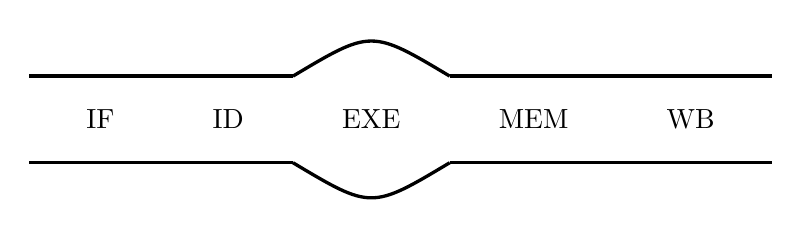
\begin{tikzpicture}[stage/.style={font=\bfseries, inner sep=1pt}]
            %--- stage labels (center line) ---
            \node (IF)  {IF};
            \node (ID)  [right=of IF]  {ID};
            \node (EXE) [right=of ID]  {EXE};
            \node (MEM) [right=of EXE] {MEM};
            \node (WB)  [right=of MEM] {WB};

            % vertical offset of the rails
            \def\dy{0.55}
            % small horizontal margin at the ends
            \def\marg{0.6}
            
            % helper points for where the bump starts/ends (midpoints around EXE)
            \coordinate (LT) at ($(ID.east)!0.5!(EXE.west)$);
            \coordinate (RT) at ($(EXE.east)!0.5!(MEM.west)$);

            %---- TOP rail: left segment, bump, right segment
            \draw[very thick] ($(IF.west)+(-\marg,\dy)$) -- ($(LT)+(0,\dy)$);
            \draw[very thick] ($(LT)+(0,\dy)$)
                .. controls ($(EXE.north)+(0,0.9)$) ..
                ($(RT)+(0,\dy)$);
            \draw[very thick] ($(RT)+(0,\dy)$) -- ($(WB.east)+(\marg,\dy)$);

            %---- BOTTOM rail: left segment, bump (down), right segment
            \draw[very thick] ($(IF.west)+(-\marg,-\dy)$) -- ($(LT)+(0,-\dy)$);
            \draw[very thick] ($(LT)+(0,-\dy)$)
                .. controls ($(EXE.south)+(0,-0.9)$) ..
                ($(RT)+(0,-\dy)$);
            \draw[very thick] ($(RT)+(0,-\dy)$) -- ($(WB.east)+(\marg,-\dy)$);
        \end{tikzpicture}
   % \end{columns}

    \begin{itemize}
        \item If we allow multiple instructions to execute in parallel in \textbf{all stages}, we can break this barrier
    \end{itemize}

    \centering
    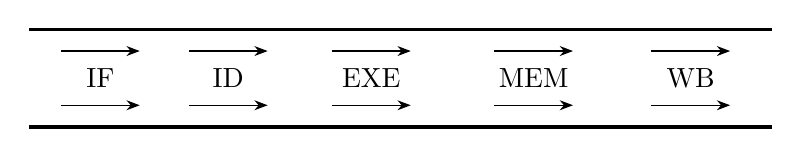
\begin{tikzpicture}[stage/.style={font=\bfseries, inner sep=1pt}]
        %--- stage labels (center line) ---
        \node (IF)  {IF};
        \node (ID)  [right=of IF]  {ID};
        \node (EXE) [right=of ID]  {EXE};
        \node (MEM) [right=of EXE] {MEM};
        \node (WB)  [right=of MEM] {WB};

        \def\dy{0.62}
        \def\dyarrowx{0.5cm}
        \def\dyarrowy{0.1cm}
        \def\marg{0.6}

        % rails
        \draw[very thick] ($(IF.west)+(-\marg,\dy)$) -- ($(WB.east)+(\marg,\dy)$);
        \draw[very thick] ($(IF.west)+(-\marg,-\dy)$) -- ($(WB.east)+(\marg,-\dy)$);
        
        \foreach \a in {IF,ID,EXE,MEM,WB}{
            \draw[-{Stealth}]
                ($(\a.north)+(-\dyarrowx,\dyarrowy)$) --
                ($(\a.north)+(\dyarrowx,\dyarrowy)$);
            \draw[-{Stealth}]
                ($(\a.south)+(-\dyarrowx,-\dyarrowy)$) --
                ($(\a.south)+(\dyarrowx,-\dyarrowy)$);
        }

    \end{tikzpicture}


    \vspace{0.5cm}
    \centering

\end{frame}

\begin{frame}{True Dependencies: RAW Hazards}
    \begin{exampleblock}{Read After Write (RAW)}
        {\ttfamily\footnotesize
        (1) ADD \textcolor{red}{R1}, R2, R3\\
        (2) ADD R5, R6, \textcolor{red}{R1}  // Must wait for \textcolor{red}{R1}
        }
    \end{exampleblock}
    
    \begin{alertblock}{Key Point}
        RAW hazards represent \textbf{true data dependencies} that cannot be eliminated—only the data flow defines program correctness.
    \end{alertblock}
\end{frame}

\begin{frame}{False Dependencies: WAR Hazards}
    \begin{exampleblock}{Write After Read (WAR)}
        {\ttfamily\footnotesize
        (1) DIV R1, R2, R3  // 40 cycles\\
        (2) ADD R5, \textcolor{red}{R6}, R1  // Waits for R1\\
        (3) ADD \textcolor{red}{R6}, R7, R8  // Could execute early!
        }
    \end{exampleblock}
    
    \begin{block}{The Problem}
        If (3) executes before (2), instruction (2) reads the \textbf{wrong} \textcolor{red}{R6} value.
    \end{block}
    
    \begin{alertblock}{Key Insight}
        WAR hazards are \textbf{artificial}—caused by register name reuse, not data flow.
    \end{alertblock}
\end{frame}

\begin{frame}{False Dependencies: WAW Hazards}
    \begin{exampleblock}{Write After Write (WAW)}
        {\ttfamily\footnotesize
        (1) DIV R1, R2, R3  // 40 cycles\\
        (2) ADD \textcolor{red}{R5}, R6, R1  // Waits for R1\\
        (3) ADD \textcolor{red}{R5}, R7, R8  // Could execute early!
        }
    \end{exampleblock}
    
    \begin{block}{The Problem}
        If (3) executes before (2), \textcolor{red}{R5} gets the \textbf{wrong} final value.
    \end{block}
    
    \begin{alertblock}{Solution Preview}
        Both WAR and WAW are \textbf{false dependencies}—register renaming eliminates them entirely.
    \end{alertblock}
\end{frame}

\begin{frame}{Register Renaming: Eliminating False Dependencies}
    \begin{block}{The Mechanism}
        \begin{itemize}
            \item \textbf{Architectural registers:} What the program sees (R0-R31)
            \item \textbf{Physical registers:} What the hardware uses (more than architectural)
        \end{itemize}
    \end{block}

    \vspace{-0.2cm}
    \textbf{Example:}

    {\ttfamily\small
    \textcolor{red}{R1} $\leftarrow$ R2+R3  $\Rightarrow$  \textcolor{correctgreen}{P17} $\leftarrow$ P5+P8\\
    \textcolor{red}{R1} $\leftarrow$ R4+R5  $\Rightarrow$  \textcolor{correctgreen}{P23} $\leftarrow$ P11+P14
    }

    \vspace{0.1cm}
    $\Rightarrow$ No WAR or WAW hazards—different physical registers for each write!

    \vspace{0cm}
    \begin{block}{Dynamic Mapping - Implementation Approaches}
        \begin{itemize}
            \item \textbf{ROB-based (Data-in-ROB):} ROB entries serve as physical registers
            \item \textbf{PRF-based (Explicit):} Separate Physical Register File
            \item \textbf{In this course:} We focus on ROB-based using \textbf{RBx} notation (RB0, RB1, ...)
        \end{itemize}
    \end{block}
\end{frame}

\begin{frame}{Register Renaming - Implementation}
    We maintain two mappings:

    \begin{enumerate}
        \item \textbf{Architectural to Physical:} (e.g., R5 to RB2)
        \begin{itemize}
            \item For resolving false dependencies
            \item Stored in \textbf{RAT} (Register Alias Table)
            \item Updated at decode stage
        \end{itemize}

        \item \textbf{Physical to Architectural:} (e.g., RB2 to R5)
        \begin{itemize}
            \item For writing the value back to the intended architectural register
            \item Stored in \textbf{ROB} (Re-Order Buffer)
            \item Used at commit/retire stage
        \end{itemize}
    \end{enumerate}
\end{frame}

\begin{frame}{OOO Execution Processor Architecture}
    \centering
    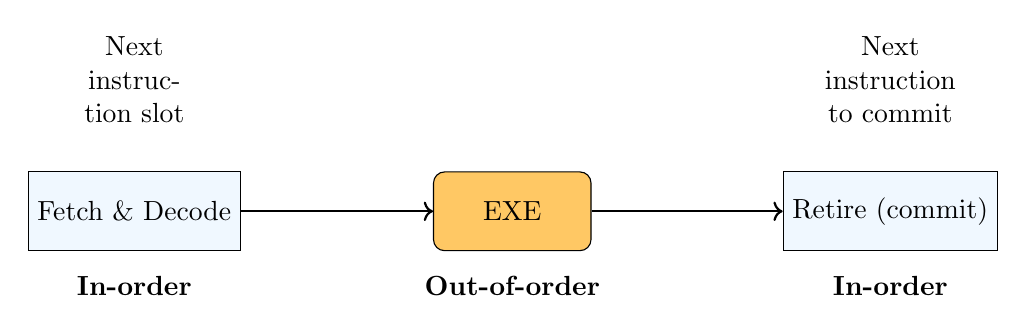
\begin{tikzpicture}[scale=1.2]
        % Stages
        \node[draw, fill=lightblue, minimum width=2cm, minimum height=1cm] (fetch) at (0,0) {Fetch \& Decode};
        \node[draw, fill=highlightorange, minimum width=2cm, minimum height=1cm, rounded corners] (exe) at (4,0) {EXE};
        \node[draw, fill=lightblue, minimum width=2cm, minimum height=1cm] (retire) at (8,0) {Retire (commit)};
        
        % Labels
        \node[below=0.2cm of fetch] {\textbf{In-order}};
        \node[below=0.2cm of exe] {\textbf{Out-of-order}};
        \node[below=0.2cm of retire] {\textbf{In-order}};
        
        % Arrows
        \draw[->, thick] (fetch) -- (exe);
        \draw[->, thick] (exe) -- (retire);
        
        % Annotations
        \node[above=0.5cm of fetch, text width=2cm, align=center] {Next instruction slot};
        \node[above=0.5cm of retire, text width=2cm, align=center] {Next instruction to commit};
    \end{tikzpicture}
    
    \vspace{0.5cm}
    Most modern processors perform fetch/decode and commit stages \textbf{in-order}, while only the execution stage is \textbf{out-of-order}.
\end{frame}

\begin{frame}{ROB (Re-Order Buffer)}
    \textbf{Purpose:} Maintain in-order commit despite out-of-order execution

    \vspace{0.3cm}

    \begin{itemize}
        \item \textbf{Allocation:} Instructions allocated to ROB entries at decode (in-order)
        \item \textbf{Physical register:} ROB entry ID serves as physical register name
        \item \textbf{Write result:} Execution units write results to ROB entries
        \item \textbf{In-order commit:} Instructions commit only when at ROB head and complete
    \end{itemize}

    \vspace{0.3cm}
    \centering
    \drawROB{
        RB0 \& R2/R3 \\
        RB1 \& R4+RB0 \\
        RB2 \& R3+R3 \\
        RB3 \& R3+RB2 \\
        : \& : \\
        RBn \& {} \\
    }
\end{frame}

\section{Question 2: ROB}

\begin{frame}{Q2a: Identify Dependencies}
    \begin{columns}[T]
        \column{0.35\textwidth}
        \textbf{Given code:}

        \vspace{0.3cm}
        {\ttfamily\small
        (1) DIV R1, R2, R3\\
        (2) ADD R2, R4, R1\\
        (3) ADD R2, R3, R3\\
        (4) ADD R4, R3, R2
        }

        \vspace{0.5cm}
        \textbf{Question:} What false dependencies exist?

        \column{0.65\textwidth}
        \only<2->{
            \begin{columns}
                \column{0.5\textwidth}
                \centering
                \textbf{WAW on R2}

                \vspace{0.2cm}

                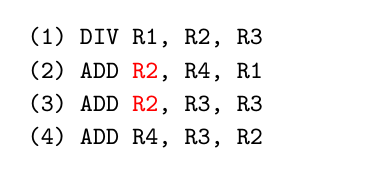
\begin{tikzpicture}[remember picture]
                    \node[anchor=north west, inner sep=0pt] (code1) {
                        \begin{minipage}{4.2cm}
                        {\ttfamily\small
                        (1) DIV R1, R2, R3\\
                        (2) ADD \tikz[remember picture, baseline=(r2a.base)]{\node[inner sep=0pt] (r2a) {\textcolor{red}{R2}};}, R4, R1\\
                        (3) ADD \tikz[remember picture, baseline=(r2b.base)]{\node[inner sep=0pt] (r2b) {\textcolor{red}{R2}};}, R3, R3\\
                        (4) ADD R4, R3, R2
                        }
                        \end{minipage}
                    };
                \end{tikzpicture}

                \begin{tikzpicture}[remember picture, overlay]
                    \draw[->, red, very thick] (r2a.east) to[bend left=40] (r2b.east);
                \end{tikzpicture}

                \column{0.5\textwidth}
                \centering
                \textbf{WAR on R4}

                \vspace{0.2cm}

                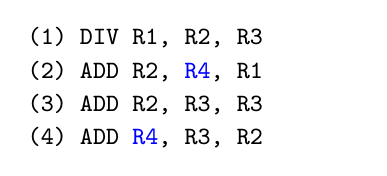
\begin{tikzpicture}[remember picture]
                    \node[anchor=north west, inner sep=0pt] (code2) {
                        \begin{minipage}{4.2cm}
                        {\ttfamily\small
                        (1) DIV R1, R2, R3\\
                        (2) ADD R2, \tikz[remember picture, baseline=(r4a.base)]{\node[inner sep=0pt] (r4a) {\textcolor{blue}{R4}};}, R1\\
                        (3) ADD R2, R3, R3\\
                        (4) ADD \tikz[remember picture, baseline=(r4b.base)]{\node[inner sep=0pt] (r4b) {\textcolor{blue}{R4}};}, R3, R2
                        }
                        \end{minipage}
                    };
                \end{tikzpicture}

                \begin{tikzpicture}[remember picture, overlay]
                    \draw[->, blue, very thick] (r4a.east) to[bend left=40] (r4b.east);
                \end{tikzpicture}
            \end{columns}

            \vspace{0.3cm}
            \textcolor{correctgreen}{\small Note: RAW dependencies (e.g., (1)$\rightarrow$(2) on R1) are true dependencies}
        }
    \end{columns}
\end{frame}

\begin{frame}{Q2b: After Decode}
    \textbf{Question:} Show the RAT and ROB state after all instructions are decoded (but before execution completes)

    \vspace{0.3cm}

    \begin{columns}[T]
        \column{0.30\textwidth}
        {\ttfamily\small
        (1) DIV R1, R2, R3\only<2->{ \checkmark}\\
        (2) ADD R2, R4, R1\only<3->{ \checkmark}\\
        (3) ADD R2, R3, R3\only<4->{ \checkmark}\\
        (4) ADD R4, R3, R2\only<5->{ \checkmark}
        }

        \vspace{0.5cm}

        \only<5->{\textcolor{correctgreen}{\small No more False Dependencies! Register renaming eliminated WAW and WAR}}

        \column{0.35\textwidth}
        \centering
        \begin{tikzpicture}[baseline=(current bounding box.north)]
            \matrix[matrix of nodes,
                    nodes={draw, minimum width=1.5cm, minimum height=0.45cm, anchor=center, font=\scriptsize},
                    column sep=-\pgflinewidth,
                    row sep=-\pgflinewidth,
                    inner sep=0pt,
                    label={above:\textbf{RAT}},
                    ampersand replacement=\&] (rat) {
                \textbf{Arch Reg} \& \textbf{Phys Reg} \\
                R1 \& \only<2->{RB0} \\
                R2 \& \only<3>{RB1}\only<4->{RB2} \\
                R3 \& {} \\
                R4 \& \only<5->{RB3} \\
            };
        \end{tikzpicture}

        \column{0.35\textwidth}
        \centering
        \begin{tikzpicture}[baseline=(current bounding box.north)]
            \matrix (rob) [matrix of nodes,
                nodes={draw, minimum width=1.5cm, minimum height=0.45cm, anchor=center, font=\scriptsize},
                row sep=-\pgflinewidth,
                column sep=-\pgflinewidth,
                inner sep=0pt,
                label={above:\textbf{ROB}},
                ampersand replacement=\&
                ] {
                RB0 \& \only<2->{R2/R3} \\
                RB1 \& \only<3->{R4+RB0} \\
                RB2 \& \only<4->{R3+R3} \\
                RB3 \& \only<5->{R3+RB2} \\
                : \& : \\
                RBn \& {} \\
            };
        \end{tikzpicture}
    \end{columns}
\end{frame}

\begin{frame}{OOO Scheme Overview}
    \centering
    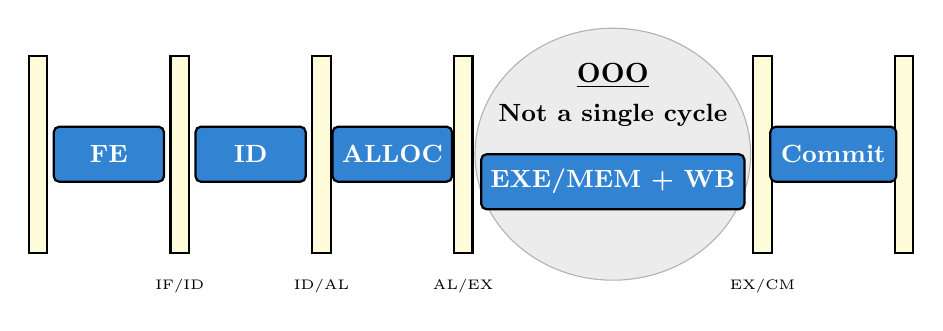
\begin{tikzpicture}[
        latch/.style={draw, thick, fill=yellow!15, minimum width=0.2cm, minimum height=2.5cm},
        stage/.style={draw, thick, fill=darkblue!80, text=white, minimum width=1.4cm, minimum height=0.7cm, font=\small\bfseries, rounded corners=2pt},
    ]
        % OOO ellipse (drawn first so it's behind everything)
        \node[draw=gray!60, fill=gray!15, ellipse, minimum width=3.5cm, minimum height=3.2cm] (ooo) at (7.3,0) {};
        \node[font=\bfseries] at (7.3,1.0) {\underline{OOO}};
        \node[font=\small\bfseries] at (7.3,0.5) {Not a single cycle};

        % Latches
        \node[latch] (L0) at (0,0) {};
        \node[latch] (L1) at (1.8,0) {};
        \node[latch] (L2) at (3.6,0) {};
        \node[latch] (L3) at (5.4,0) {};
        \node[latch] (L4) at (9.2,0) {};
        \node[latch] (L5) at (11.0,0) {};

        % Stage boxes
        \node[stage] (fe) at (0.9,0) {FE};
        \node[stage] (id) at (2.7,0) {ID};
        \node[stage] (alloc) at (4.5,0) {ALLOC};
        \node[stage, minimum width=2.2cm] (exe) at (7.3,-0.35) {EXE/MEM + WB};
        \node[stage, minimum width=1.6cm] (commit) at (10.1,0) {Commit};

        % Labels below latches
        \node[below=2mm of L1, font=\tiny] {IF/ID};
        \node[below=2mm of L2, font=\tiny] {ID/AL};
        \node[below=2mm of L3, font=\tiny] {AL/EX};
        \node[below=2mm of L4, font=\tiny] {EX/CM};
    \end{tikzpicture}
\end{frame}

\begin{frame}{Historical Note: IBM System/360 Model 91 (1966)}
    \begin{columns}
        \column{0.4\textwidth}
        \includegraphics[width=\textwidth]{figures/ibm360m91.jpg}

        \vspace{0.2cm}
        \scriptsize Photo: NASA Goddard Space Flight Center
        {
            \fontsize{4}{5}\selectfont
            By Bundesarchiv, B 145 Bild-F038812-0014 / Schaack, Lothar /
            \href{https://commons.wikimedia.org/w/index.php?curid=5455799}{CC-BY-SA 3.0}
        }

        \column{0.6\textwidth}
        \begin{itemize}
            \item \textbf{First IBM computer} with out-of-order execution
            \item Developed by Robert Tomasulo at IBM
            \item Introduced the \textbf{Tomasulo Algorithm}:
            \begin{itemize}
                \footnotesize
                \item Register renaming via reservation stations
                \item Dynamic scheduling
                \item Common Data Bus (CDB) for results
            \end{itemize}
            \item \textbf{Performance:} 16.6 MFLOPS peak
            \item \textbf{Cost:} \$6-7 million (1966 dollars)
        \end{itemize}
    \end{columns}

    \vspace{0.3cm}
    \begin{alertblock}{Legacy}
        The Tomasulo algorithm's concepts remain fundamental to modern processors—every high-performance CPU today uses variations of these techniques.
    \end{alertblock}
\end{frame}

\section{Question 3: OOO Execution Trace}

\begin{frame}{OOO Execution Structures (Review)}
    \textbf{Key Data Structures for Out-of-Order Execution:}

    \begin{itemize}
        \item \textbf{RAT (Register Alias Table):} Maps architectural registers to physical registers (ROB entries)
        \item \textbf{ROB (Re-Order Buffer):} Circular buffer maintaining program order; also holds physical register values
        \item \textbf{RRF (Retire Register File):} Holds committed architectural register values
        \item \textbf{RS (Reservation Station):} Holds decoded instructions waiting for operands
        \item \textbf{MOB (Memory Order Buffer):} Manages memory operations in order
        \item \textbf{IDQ (Instruction Decode Queue):} Holds fetched instructions
    \end{itemize}
\end{frame}

\begin{frame}{Structure Interaction (Intel CPUs)}
    \begin{tikzpicture}[font=\tiny, remember picture, overlay]
        % Explanation box in top left corner of page - minimal offset
        \node[draw, fill=yellow!10, inner sep=5pt, text width=4.5cm, align=left, anchor=north west] at ([xshift=0.2cm, yshift=-1.5cm]current page.north west) {
            \tiny
            \only<1>{
            \textbf{Instructions Flow:}\\[0.1cm]
            IDQ $\rightarrow$ RAT (decode/rename) $\rightarrow$ ROB \& RS (track \& wait) $\rightarrow$ Execute\\[0.2cm]

            \textbf{Physical Registers:}\\[0.05cm]
            Phys Reg entries (ROB\#) referenced by:\\
            - RAT: points to ROB entry\\
            - RS.Pdst: destination ROB entry\\
            - RS.srcX (valid=0): waiting for ROB entry
            }
            \only<2->{
            \textbf{ROB Entries:}\\[0.05cm]
            - If Alloc=I: entry not allocated, rest meaningless\\
            - If Data Valid=I: value meaningless\\
            - Arch Reg: for writeback at retire\\[0.2cm]

            \textbf{RS Operation:}\\[0.05cm]
            - RRF values: ready immediately\\
            - ROB values: ready once execution unit produces result
            }
        };
    \end{tikzpicture}

    \centering
    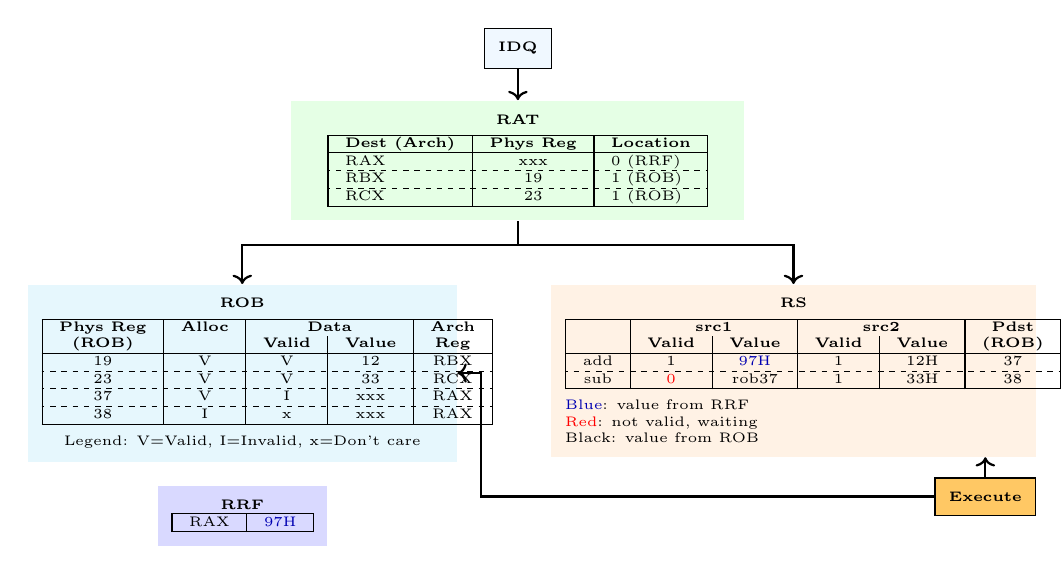
\begin{tikzpicture}[font=\tiny]
        % IDQ at top
        \node[draw, fill=lightblue, inner sep=5pt] (idq) {\textbf{IDQ}};

        % RAT below IDQ
        \node[fill=green!10, inner sep=5pt, below=0.4cm of idq] (rat) {
            \begin{minipage}{5.4cm}
            \centering
            \textbf{RAT}

            \vspace{0.1cm}
            \tiny
            \begin{tabular}{|l|c|l|}
            \hline
            \textbf{Dest (Arch)} & \textbf{Phys Reg} & \textbf{Location} \\
            \hline
            RAX & xxx & 0 (RRF) \\
            \hdashline[2pt/2pt]
            RBX & 19 & 1 (ROB) \\
            \hdashline[2pt/2pt]
            RCX & 23 & 1 (ROB) \\
            \hline
            \end{tabular}
            \end{minipage}
        };

        % ROB below and left of RAT
        \node[fill=cyan!10, inner sep=5pt, below=0.8cm of rat.south, anchor=north, xshift=-3.5cm] (rob) {
            \begin{minipage}{5.1cm}
            \centering
            \textbf{ROB}

            \vspace{0.1cm}
            \tiny
            \begin{tabular}{|c|c|c|c|c|}
            \hline
            \textbf{Phys Reg} & \textbf{Alloc} & \multicolumn{2}{c|}{\textbf{Data}} & \textbf{Arch} \\
            \textbf{(ROB)} & & \textbf{Valid} & \textbf{Value} & \textbf{Reg} \\
            \hline
            19 & V & V & 12 & RBX \\
            \hdashline[2pt/2pt]
            23 & V & V & 33 & RCX \\
            \hdashline[2pt/2pt]
            37 & V & I & xxx & RAX \\
            \hdashline[2pt/2pt]
            38 & I & x & xxx & RAX \\
            \hline
            \end{tabular}

            \vspace{0.1cm}
            \tiny
            Legend: V=Valid, I=Invalid, x=Don't care
            \end{minipage}
        };

        % RS below and right of RAT
        \node[fill=orange!10, inner sep=5pt, below=0.8cm of rat.south, anchor=north, xshift=3.5cm] (rs) {
            \begin{minipage}{5.8cm}
            \centering
            \textbf{RS}

            \vspace{0.1cm}
            \tiny
            \begin{tabular}{|c|c|c|c|c|c|}
            \hline
             & \multicolumn{2}{c|}{\textbf{src1}} & \multicolumn{2}{c|}{\textbf{src2}} & \textbf{Pdst} \\
             & \textbf{Valid} & \textbf{Value} & \textbf{Valid} & \textbf{Value} & \textbf{(ROB)} \\
            \hline
            add & 1 & \textcolor{blue!70!black}{97H} & 1 & 12H & 37 \\
            \hdashline[2pt/2pt]
            sub & \textcolor{red}{0} & rob37 & 1 & 33H & 38 \\
            \hline
            \end{tabular}

            \vspace{0.1cm}
            \raggedright
            \tiny
            \textcolor{blue!70!black}{Blue}: value from RRF\\
            \textcolor{red}{Red}: not valid, waiting\\
            Black: value from ROB
            \end{minipage}
        };

        % RRF below ROB
        \node[fill=blue!15, inner sep=5pt, below=0.3cm of rob.south, anchor=north] (rrf) {
            \begin{minipage}{1.8cm}
            \centering
            \tiny
            \textbf{RRF}
            \begin{tabular}{|c|c|}
            \hline
            RAX & \textcolor{blue!70!black}{97H} \\
            \hline
            \end{tabular}
            \end{minipage}
        };

        % Execute below RS and ROB
        \node[draw, fill=highlightorange, inner sep=5pt, below=0.5cm of rs.south east, anchor=east] (execute) {\textbf{Execute}};

        % Arrows
        \draw[->, thick] (idq.south) -- (rat.north);
        \draw[->, thick] (rat.south) -- ++(0,-0.3) -| (rob.north);
        \draw[->, thick] (rat.south) -- ++(0,-0.3) -| (rs.north);
        \draw[->, thick] (execute.north) -- (rs.south -| execute.north);
        \draw[->, thick] (execute.west) -| ([xshift=3mm]rob.east) -- (rob.east);

    \end{tikzpicture}
\end{frame}

\begin{frame}{Simplified Notation for Trace}
    For the cycle-by-cycle trace, we'll use simplified notation:

    \vspace{0.3cm}
    \begin{itemize}
        \item \textbf{RAT:} Show only Arch Reg $\rightarrow$ Phys Reg mapping (omit source column)
        \item \textbf{ROB:} Show only operation and status (INV/OK), omit detailed valid bits and data values
        \item \textbf{RS:} Show operation with dependencies (e.g., RB0$\leftarrow$R4/R3)
        \item \textbf{Execute:} Show operation with remaining cycles in brackets
    \end{itemize}

    \vspace{0.3cm}
    This simplification helps focus on the key concepts: \textbf{register renaming, dependency tracking, and out-of-order execution}.
\end{frame}

\begin{frame}{Q3: How Does OOO Execution Work Cycle-by-Cycle?}
    \textbf{Question:} How many cycles will it take to execute the following program using out-of-order execution?

    \textit{Assume all instructions have already been decoded and are in the IDQ.}

    \vspace{0.4cm}
    \begin{columns}[T]
        \begin{column}{0.5\textwidth}
            \textbf{Program:}

            {\ttfamily\small
            \begin{tabular}{ll}
            (1) & DIV R2, R4, R3 \\
            (2) & LD R3, R4(50) \\
            (3) & DIV R1, R2, R3 \\
            (4) & ADD R2, R4, R3 \\
            (5) & SUB R3, R2, R3 \\
            \end{tabular}
            }
        \end{column}
        \begin{column}{0.45\textwidth}
            \textbf{Latencies:}

            \begin{itemize}
                \item \textbf{DIV:} 4 cycles
                \item \textbf{LD:} 2 cycles
                \item \textbf{ADD/SUB:} 1 cycle
            \end{itemize}
        \end{column}
    \end{columns}

    \vspace{0.4cm}
    \textbf{Observation:} Instructions (1) and (2) are independent and can execute in parallel. Instruction (3) depends on both (1) and (2).
\end{frame}

\begin{frame}{Notation for Cycle-by-Cycle Walkthrough}
    \begin{block}{Execution Status Notation}
        In the \textbf{Execute} section, we show operations currently being executed with their \textbf{remaining cycle count} in brackets.

        \vspace{0.3cm}
        \textbf{Example:} RB0$\leftarrow$R4/R3 [3]
        \begin{itemize}
            \item This means ROB entry RB0 is executing the DIV operation R4/R3
            \item There are \textbf{3 cycles remaining} until this operation completes
            \item Next cycle, this will show [2], then [1], then complete
        \end{itemize}
    \end{block}

    \vspace{0.2cm}
    \textbf{Operation Latencies (Reminder):}
    \begin{itemize}
        \item DIV: 4 cycles $\rightarrow$ shows [4], [3], [2], [1]
        \item LD: 2 cycles $\rightarrow$ shows [2], [1]
        \item ADD/SUB: 1 cycle $\rightarrow$ shows [1]
    \end{itemize}
\end{frame}

\begin{frame}{Cycle 1: Decode}
    \centering
    \OOODiagram[
        R1={}, R2={\newentrya{RB0}}, R3={}, R4={},
        rob01={\newentrya{R2$\leftarrow$R4/R3}}, rob02={\newentrya{INV}},
        rs1={\newentrya{RB0$\leftarrow$R4/R3}},
        instq1={SUB R3,R2,R3}, instq2={ADD R2,R4,R3}, instq3={DIV R1,R2,R3}, instq4={LD R3,R4(50)}, instq5={\newentrya{\sout{DIV R2,R4,R3}}}
    ]

    \vspace{0.3cm}
    \begin{tikzpicture}[remember picture, overlay]
        \node[anchor=south west, text width=6cm, font=\small, xshift=0.5cm, yshift=0.5cm] at (current page.south west) {
            \begin{block}{What's Happening}
                First instruction (DIV R2,R4,R3) is decoded. RAT maps R2 to RB0, ROB allocates RB0, and RS receives the operation with operands ready.
            \end{block}
        };
    \end{tikzpicture}
\end{frame}

\begin{frame}{Cycle 2: Execute}
    \centering
    \OOODiagram[
        R1={}, R2={\oldentry{RB0}}, R3={}, R4={},
        rob01={\oldentry{R2$\leftarrow$R4/R3}}, rob02={\oldentry{INV}},
        rs1={\srcentrya{\sout{RB0$\leftarrow$R4/R3}}},
        exec1={\newentrya{RB0$\leftarrow$R4/R3 [4]}},
        instq1={SUB R3,R2,R3}, instq2={ADD R2,R4,R3}, instq3={DIV R1,R2,R3}, instq4={LD R3,R4(50)}, instq5={~}
    ]

    \vspace{0.3cm}
    \begin{tikzpicture}[remember picture, overlay]
        \node[anchor=south west, text width=6cm, font=\small, xshift=0.5cm, yshift=0.5cm] at (current page.south west) {
            \begin{block}{What's Happening}
                RB0 (DIV) dispatched from RS to execution unit. DIV takes 4 cycles, shown as [4].
            \end{block}
        };
    \end{tikzpicture}
\end{frame}

\begin{frame}{Cycle 2: Decode}
    \centering
    \OOODiagram[
        R1={}, R2={\oldentry{RB0}}, R3={\newentrya{RB1}}, R4={},
        rob01={\oldentry{R2$\leftarrow$R4/R3}}, rob02={\oldentry{INV}},
        rob11={\newentrya{R3$\leftarrow$LD R4(50)}}, rob12={\newentrya{INV}},
        rs1={\newentrya{MOB$\leftarrow$R4+50}},
        exec1={\oldentry{RB0$\leftarrow$R4/R3 [4]}},
        mob1={\newentrya{RB1$\leftarrow$MEM(?) [W]}},
        instq1={SUB R3,R2,R3}, instq2={ADD R2,R4,R3}, instq3={DIV R1,R2,R3}, instq4={\srcentrya{\sout{LD R3,R4(50)}}}, instq5={~}
    ]

    \vspace{0.3cm}
    \begin{tikzpicture}[remember picture, overlay]
        \node[anchor=south west, text width=6cm, font=\small, xshift=0.5cm, yshift=0.5cm] at (current page.south west) {
            \begin{block}{What's Happening}
                LD decoded: RAT maps R3 to RB1, ROB allocates RB1. MOB entry created with [W] - waiting for address R4+50 to be computed.
            \end{block}
        };
    \end{tikzpicture}
\end{frame}

\begin{frame}{Cycle 3: Execute}
    \centering
    \OOODiagram[
        R1={}, R2={\oldentry{RB0}}, R3={\oldentry{RB1}}, R4={},
        rob01={\oldentry{R2$\leftarrow$R4/R3}}, rob02={\oldentry{INV}},
        rob11={\oldentry{R3$\leftarrow$LD R4(50)}}, rob12={\oldentry{INV}},
        exec1={\newentrya{RB0$\leftarrow$R4/R3 [3]}},
        exec2={\newentryb{MOB$\leftarrow$R4+50}},
        mob1={\oldentry{RB1$\leftarrow$MEM(?) [W]}},
        instq1={SUB R3,R2,R3}, instq2={ADD R2,R4,R3}, instq3={DIV R1,R2,R3}, instq4={~}, instq5={~}
    ]

    \vspace{0.3cm}
    \begin{tikzpicture}[remember picture, overlay]
        \node[anchor=south west, text width=6cm, font=\small, xshift=0.5cm, yshift=0.5cm] at (current page.south west) {
            \begin{block}{What's Happening}
                RB0 continues executing [4$\rightarrow$3]. Address R4+50 computed (ADD takes 1 cycle). MOB still waiting [W] for address to complete.
            \end{block}
        };
    \end{tikzpicture}
\end{frame}

\begin{frame}{Cycle 3: Decode}
    \centering
    \OOODiagram[
        R1={\newentrya{RB2}}, R2={\oldentry{RB0}}, R3={\oldentry{RB1}}, R4={},
        rob01={\oldentry{R2$\leftarrow$R4/R3}}, rob02={\oldentry{INV}},
        rob11={\oldentry{R3$\leftarrow$LD R4(50)}}, rob12={\oldentry{INV}},
        rob21={\newentrya{R1$\leftarrow$RB0/RB1}}, rob22={\newentrya{INV}},
        rs2={\newentrya{RB2$\leftarrow$\textcolor{red}{RB0}/\textcolor{red}{RB1}}},
        exec1={\oldentry{RB0$\leftarrow$R4/R3 [3]}},
        exec2={\oldentry{MOB$\leftarrow$R4+50}},
        mob1={\oldentry{RB1$\leftarrow$MEM(?) [W]}},
        instq1={SUB R3,R2,R3}, instq2={ADD R2,R4,R3}, instq3={\srcentrya{\sout{DIV R1,R2,R3}}}, instq4={~}, instq5={~}
    ]

    \vspace{0.3cm}
    \begin{tikzpicture}[remember picture, overlay]
        \node[anchor=south west, text width=6cm, font=\small, xshift=0.5cm, yshift=0.5cm] at (current page.south west) {
            \begin{block}{What's Happening}
                DIV R1 decoded - depends on RB0 and RB1, goes to RS but can't execute yet. LD now dispatched from MOB with [2] cycles. RB0 continues at [3].
            \end{block}
        };
    \end{tikzpicture}
\end{frame}

\begin{frame}{Cycle 4: Execute}
    \centering
    \OOODiagram[
        R1={\oldentry{RB2}}, R2={\oldentry{RB3}}, R3={\oldentry{RB1}}, R4={},
        rob01={\oldentry{R2$\leftarrow$R4/R3}}, rob02={\oldentry{INV}},
        rob11={\oldentry{R3$\leftarrow$LD R4(50)}}, rob12={\oldentry{INV}},
        rob21={\oldentry{R1$\leftarrow$RB0/RB1}}, rob22={\oldentry{INV}},
        rob31={\oldentry{R2$\leftarrow$R4+RB1}}, rob32={\oldentry{INV}},
        rs2={\oldentry{RB2$\leftarrow$\textcolor{red}{RB0}/\textcolor{red}{RB1} [W]}},
        rs3={\oldentry{RB3$\leftarrow$R4+\textcolor{red}{RB1} [W]}},
        exec1={\newentrya{RB0$\leftarrow$R4/R3 [2]}},
        exec2={\srcentryb{\sout{MOB$\leftarrow$R4+50}}},
        mob1={\newentryb{RB1$\leftarrow$R4(50) [2]}},
        instq1={SUB R3,R2,R3}, instq2={ADD R2,R4,R3}, instq3={~}, instq4={~}, instq5={~}
    ]

    \vspace{0.3cm}
    \begin{tikzpicture}[remember picture, overlay]
        \node[anchor=south west, text width=6cm, font=\small, xshift=0.5cm, yshift=0.5cm] at (current page.south west) {
            \begin{block}{What's Happening}
                RB0 (DIV) at [3]. RB1 (LD) completes - last cycle [1]. ROB will be marked OK after this cycle.
            \end{block}
        };
    \end{tikzpicture}
\end{frame}

\begin{frame}{Cycle 4: Decode}
    \centering
    \OOODiagram[
        R1={\oldentry{RB2}}, R2={\newentrya{RB3}}, R3={\oldentry{RB1}}, R4={},
        rob01={\oldentry{R2$\leftarrow$R4/R3}}, rob02={\oldentry{INV}},
        rob11={\oldentry{R3$\leftarrow$LD R4(50)}}, rob12={\oldentry{INV}},
        rob21={\oldentry{R1$\leftarrow$RB0/RB1}}, rob22={\oldentry{INV}},
        rob31={\newentrya{R2$\leftarrow$R4+RB1}}, rob32={\newentrya{INV}},
        rs2={\oldentry{RB2$\leftarrow$\textcolor{red}{RB0}/\textcolor{red}{RB1} [W]}},
        rs3={\newentrya{RB3$\leftarrow$R4+\textcolor{red}{RB1} [W]}},
        exec1={\oldentry{RB0$\leftarrow$R4/R3 [2]}},
        mob1={\oldentry{RB1$\leftarrow$R4(50) [2]}},
        instq1={SUB R3,R2,R3}, instq2={\srcentrya{\sout{ADD R2,R4,R3}}}, instq3={~}, instq4={~}, instq5={~}
    ]

    \vspace{0.3cm}
    \begin{tikzpicture}[remember picture, overlay]
        \node[anchor=south west, text width=6cm, font=\small, xshift=0.5cm, yshift=0.5cm] at (current page.south west) {
            \begin{block}{What's Happening}
                ADD decoded: RAT maps R2 to RB3 (old RB0 still in ROB). RS entry waits for RB1. RB1 completes, ROB marked OK. RB0 at [3].
            \end{block}
        };
    \end{tikzpicture}
\end{frame}

\begin{frame}{Cycle 5: Execute}
    \centering
    \OOODiagram[
        R1={\oldentry{RB2}}, R2={\oldentry{RB3}}, R3={\oldentry{RB1}}, R4={},
        rob01={\oldentry{R2$\leftarrow$R4/R3}}, rob02={\oldentry{INV}},
        rob11={\oldentry{R3$\leftarrow$LD R4(50)}}, rob12={\oldentry{INV}},
        rob21={\oldentry{R1$\leftarrow$RB0/RB1}}, rob22={\oldentry{INV}},
        rob31={\oldentry{R2$\leftarrow$R4+RB1}}, rob32={\oldentry{INV}},
        rs2={\oldentry{RB2$\leftarrow$\textcolor{red}{RB0}/\textcolor{red}{RB1} [W]}},
        rs3={\oldentry{RB3$\leftarrow$R4+\textcolor{red}{RB1} [W]}},
        exec1={\newentrya{RB0$\leftarrow$R4/R3 [1]}},
        mob1={\newentrya{RB1$\leftarrow$R4(50) [1]}},
        instq1={SUB R3,R2,R3}, instq2={~}, instq3={~}, instq4={~}, instq5={~}
    ]

    \vspace{0.3cm}
    \begin{tikzpicture}[remember picture, overlay]
        \node[anchor=south west, text width=6cm, font=\small, xshift=0.5cm, yshift=0.5cm] at (current page.south west) {
            \begin{block}{What's Happening}
                RB0 (DIV) at [1]. RS blocked: RB2 waiting [W] on RB0 and RB1 dependencies, cannot dispatch. MOB at [1]. Retirement stalled waiting for RB0 to complete.
            \end{block}
        };
    \end{tikzpicture}
\end{frame}

\begin{frame}{Cycle 5: Decode}
    \centering
    \OOODiagram[
        R1={\oldentry{RB2}}, R2={\oldentry{RB3}}, R3={\newentrya{RB4}}, R4={},
        rob01={\oldentry{R2$\leftarrow$R4/R3}}, rob02={\oldentry{INV}},
        rob11={\oldentry{R3$\leftarrow$LD R4(50)}}, rob12={\oldentry{INV}},
        rob21={\oldentry{R1$\leftarrow$RB0/RB1}}, rob22={\oldentry{INV}},
        rob31={\oldentry{R2$\leftarrow$R4+RB1}}, rob32={\oldentry{INV}},
        rob41={\newentrya{R3$\leftarrow$RB3-RB1}}, rob42={\newentrya{INV}},
        rs1={\newentrya{RB4$\leftarrow$\textcolor{red}{RB3}-\textcolor{red}{RB1} [W]}},
        rs2={\oldentry{RB2$\leftarrow$\textcolor{red}{RB0}/\textcolor{red}{RB1} [W]}},
        rs3={\oldentry{RB3$\leftarrow$R4+\textcolor{red}{RB1} [W]}},
        exec1={\oldentry{RB0$\leftarrow$R4/R3 [1]}},
        mob1={\oldentry{RB1$\leftarrow$R4(50) [1]}},
        instq1={\srcentrya{\sout{SUB R3,R2,R3}}}, instq2={~}, instq3={~}, instq4={~}, instq5={~}
    ]

    \vspace{0.3cm}
    \begin{tikzpicture}[remember picture, overlay]
        \node[anchor=south west, text width=6cm, font=\small, xshift=0.5cm, yshift=0.5cm] at (current page.south west) {
            \begin{block}{What's Happening}
                SUB decoded, creates RB4 in ROB with dependencies on RB3 and RB1. RB4 enters RS waiting for RB3. RB3 dispatched to execute. RB0 at [2].
            \end{block}
        };
    \end{tikzpicture}
\end{frame}

\begin{frame}{Cycle 6: Execution Completes}
    \centering
    \OOODiagram[
        R1={\oldentry{RB2}}, R2={\oldentry{RB3}}, R3={\oldentry{RB4}}, R4={},
        rob01={\oldentry{R2$\leftarrow$R4/R3}}, rob02={\newentryb{OK}},
        rob11={\oldentry{R3$\leftarrow$LD R4(50)}}, rob12={\newentrya{OK}},
        rob21={\oldentry{R1$\leftarrow$RB0/RB1}}, rob22={\oldentry{INV}},
        rob31={\oldentry{R2$\leftarrow$R4+RB1}}, rob32={\oldentry{INV}},
        rob41={\oldentry{R3$\leftarrow$RB3-RB1}}, rob42={\oldentry{INV}},
        rs1={\oldentry{RB4$\leftarrow$\textcolor{red}{RB3}-\newentrya{RB1} [W]}},
        rs2={\oldentry{RB2$\leftarrow$\newentryb{RB0}/\newentrya{RB1}}},
        rs3={\oldentry{RB3$\leftarrow$R4+\newentrya{RB1}}},
        exec1={\srcentryb{\sout{RB0$\leftarrow$R4/R3}}},
        mob1={\srcentrya{\sout{RB1$\leftarrow$R4(50)}}},
        instq1={~}, instq2={~}, instq3={~}, instq4={~}, instq5={~}
    ]

    \vspace{0.3cm}
    \begin{tikzpicture}[remember picture, overlay]
        \node[anchor=south west, text width=6cm, font=\small, xshift=0.5cm, yshift=0.5cm] at (current page.south west) {
            \begin{block}{What's Happening}
                RB0 (DIV) and RB1 (LD) complete, marked OK. Forwarding: RB2 and RB3 in RS now unblocked, ready to dispatch. RB4 still waiting [W] on RB3.
            \end{block}
        };
    \end{tikzpicture}
\end{frame}

\begin{frame}{Cycle 6: Execute}
    \centering
    \OOODiagram[
        R1={\oldentry{RB2}}, R2={\oldentry{RB3}}, R3={\oldentry{RB4}}, R4={},
        rob01={\oldentry{R2$\leftarrow$R4/R3}}, rob02={\oldentry{OK}},
        rob11={\oldentry{R3$\leftarrow$LD R4(50)}}, rob12={\oldentry{OK}},
        rob21={\oldentry{R1$\leftarrow$RB0/RB1}}, rob22={\oldentry{INV}},
        rob31={\oldentry{R2$\leftarrow$R4+RB1}}, rob32={\oldentry{INV}},
        rob41={\oldentry{R3$\leftarrow$RB3-RB1}}, rob42={\oldentry{INV}},
        rs1={\oldentry{RB4$\leftarrow$\textcolor{red}{RB3}-RB1 [W]}},
        rs2={\srcentrya{\sout{RB2$\leftarrow$RB0/RB1}}},
        rs3={\srcentryb{\sout{RB3$\leftarrow$R4+RB1}}},
        exec1={\newentrya{RB2$\leftarrow$RB0/RB1 [4]}},
        exec2={\newentryb{RB3$\leftarrow$R4+RB1 [1]}},
        instq1={~}, instq2={~}, instq3={~}, instq4={~}, instq5={~}
    ]

    \vspace{0.3cm}
    \begin{tikzpicture}[remember picture, overlay]
        \node[anchor=south west, text width=6cm, font=\small, xshift=0.5cm, yshift=0.5cm] at (current page.south west) {
            \begin{block}{What's Happening}
                RB2 (DIV) and RB3 (ADD) dispatch from RS and start executing [4] and [1]. RB4 still waiting [W] on RB3. No retirement yet.
            \end{block}
        };
    \end{tikzpicture}
\end{frame}

\begin{frame}{Cycle 7: Retire}
    \centering
    \OOODiagram[
        R1={\oldentry{RB2}}, R2={\oldentry{RB3}}, R3={\oldentry{RB4}}, R4={},
        rob01={\srcentrya{\sout{R2$\leftarrow$R4/R3}}}, rob02={\srcentrya{\sout{OK}}},
        rob11={\srcentryb{\sout{R3$\leftarrow$LD R4(50)}}}, rob12={\srcentryb{\sout{OK}}},
        rob21={\oldentry{R1$\leftarrow$RB0/RB1}}, rob22={\oldentry{INV}},
        rob31={\oldentry{R2$\leftarrow$R4+RB1}}, rob32={\oldentry{INV}},
        rob41={\oldentry{R3$\leftarrow$RB3-RB1}}, rob42={\oldentry{INV}},
        rs1={\oldentry{RB4$\leftarrow$\textcolor{red}{RB3}-RB1 [W]}},
        exec1={\oldentry{RB2$\leftarrow$RB0/RB1 [4]}},
        exec2={\oldentry{RB3$\leftarrow$R4+RB1 [1]}},
        ret1={\newentrya{R2$\leftarrow$RB0}},
        ret2={\newentryb{R3$\leftarrow$RB1}},
        instq1={~}, instq2={~}, instq3={~}, instq4={~}, instq5={~}
    ]

    \vspace{0.3cm}
    \begin{tikzpicture}[remember picture, overlay]
        \node[anchor=south west, text width=6cm, font=\small, xshift=0.5cm, yshift=0.5cm] at (current page.south west) {
            \begin{block}{What's Happening}
                RB0 and RB1 retire, committing R2 and R3. ROB entries freed. RB2 continues [4], RB3 continues [1].
            \end{block}
        };
    \end{tikzpicture}
\end{frame}

\begin{frame}{Cycle 7: Execution Completes}
    \centering
    \OOODiagram[
        R1={\oldentry{RB2}}, R2={\oldentry{RB3}}, R3={\oldentry{RB4}}, R4={},
        rob21={\oldentry{R1$\leftarrow$RB0/RB1}}, rob22={\oldentry{INV}},
        rob31={\oldentry{R2$\leftarrow$R4+RB1}}, rob32={\newentrya{OK}},
        rob41={\oldentry{R3$\leftarrow$RB3-RB1}}, rob42={\oldentry{INV}},
        rs1={\oldentry{RB4$\leftarrow$\newentrya{RB3}-RB1}},
        exec1={\oldentry{RB2$\leftarrow$RB0/RB1 [4]}},
        exec2={\srcentrya{\sout{RB3$\leftarrow$R4+RB1}}},
        instq1={~}, instq2={~}, instq3={~}, instq4={~}, instq5={~}
    ]

    \vspace{0.3cm}
    \begin{tikzpicture}[remember picture, overlay]
        \node[anchor=south west, text width=6cm, font=\small, xshift=0.5cm, yshift=0.5cm] at (current page.south west) {
            \begin{block}{What's Happening}
                RB3 (ADD) completes execution. Result forwarded to RB4 in RS - RB3 dependency resolved, no longer waiting [W].
            \end{block}
        };
    \end{tikzpicture}
\end{frame}

\begin{frame}{Cycle 7: Execute}
    \centering
    \OOODiagram[
        R1={\oldentry{RB2}}, R2={\oldentry{RB3}}, R3={\oldentry{RB4}}, R4={},
        rob21={\oldentry{R1$\leftarrow$RB0/RB1}}, rob22={\oldentry{INV}},
        rob31={\oldentry{R2$\leftarrow$R4+RB1}}, rob32={\oldentry{OK}},
        rob41={\oldentry{R3$\leftarrow$RB3-RB1}}, rob42={\oldentry{INV}},
        rs1={\srcentryb{\sout{RB4$\leftarrow$RB3-RB1}}},
        exec1={\newentrya{RB2$\leftarrow$RB0/RB1 [3]}},
        exec2={\newentryb{RB4$\leftarrow$RB3-RB1 [1]}},
        instq1={~}, instq2={~}, instq3={~}, instq4={~}, instq5={~}
    ]

    \vspace{0.3cm}
    \begin{tikzpicture}[remember picture, overlay]
        \node[anchor=south west, text width=6cm, font=\small, xshift=0.5cm, yshift=0.5cm] at (current page.south west) {
            \begin{block}{What's Happening}
                RB2 (DIV) continues [3]. RB4 (SUB) dispatches from RS and starts executing [1]. Nothing to decode.
            \end{block}
        };
    \end{tikzpicture}
\end{frame}

\begin{frame}{Cycle 8: Retire}
    \centering
    \OOODiagram[
        R1={\oldentry{RB2}}, R2={\oldentry{RB3}}, R3={\oldentry{RB4}}, R4={},
        rob21={\srcentrya{R1$\leftarrow$RB0/RB1}}, rob22={\srcentrya{INV}},
        rob31={\oldentry{R2$\leftarrow$R4+RB1}}, rob32={\oldentry{OK}},
        rob41={\oldentry{R3$\leftarrow$RB3-RB1}}, rob42={\oldentry{INV}},
        exec1={\oldentry{RB2$\leftarrow$RB0/RB1 [3]}},
        exec2={\oldentry{RB4$\leftarrow$RB3-RB1 [1]}},
        instq1={~}, instq2={~}, instq3={~}, instq4={~}, instq5={~}
    ]

    \vspace{0.3cm}
    \begin{tikzpicture}[remember picture, overlay]
        \node[anchor=south west, text width=6cm, font=\small, xshift=0.5cm, yshift=0.5cm] at (current page.south west) {
            \begin{block}{What's Happening}
                No retirement can take place. RB2 is at the head of ROB but still INV (not complete). Despite RB3 being OK and ready, it cannot retire - must retire in-order.
            \end{block}
        };
    \end{tikzpicture}
\end{frame}

\begin{frame}{Cycle 8: Execute}
    \centering
    \OOODiagram[
        R1={\oldentry{RB2}}, R2={\oldentry{RB3}}, R3={\oldentry{RB4}}, R4={},
        rob21={\oldentry{R1$\leftarrow$RB0/RB1}}, rob22={\oldentry{INV}},
        rob31={\oldentry{R2$\leftarrow$R4+RB1}}, rob32={\oldentry{OK}},
        rob41={\oldentry{R3$\leftarrow$RB3-RB1}}, rob42={\newentryb{OK}},
        exec1={\newentrya{RB2$\leftarrow$RB0/RB1 [2]}},
        exec2={\srcentryb{\sout{RB4$\leftarrow$RB3-RB1}}},
        instq1={~}, instq2={~}, instq3={~}, instq4={~}, instq5={~}
    ]

    \vspace{0.3cm}
    \begin{tikzpicture}[remember picture, overlay]
        \node[anchor=south west, text width=6cm, font=\small, xshift=0.5cm, yshift=0.5cm] at (current page.south west) {
            \begin{block}{What's Happening}
                RB2 (DIV) continues [2]. RB4 (SUB) completes execution, writes result to ROB. Nothing to decode.
            \end{block}
        };
    \end{tikzpicture}
\end{frame}

\begin{frame}{Cycle 9: Retire}
    \centering
    \OOODiagram[
        R1={\oldentry{RB2}}, R2={\oldentry{RB3}}, R3={\oldentry{RB4}}, R4={},
        rob21={\srcentrya{R1$\leftarrow$RB0/RB1}}, rob22={\srcentrya{INV}},
        rob31={\oldentry{R2$\leftarrow$R4+RB1}}, rob32={\oldentry{OK}},
        rob41={\oldentry{R3$\leftarrow$RB3-RB1}}, rob42={\oldentry{OK}},
        exec1={\oldentry{RB2$\leftarrow$RB0/RB1 [2]}},
        instq1={~}, instq2={~}, instq3={~}, instq4={~}, instq5={~}
    ]

    \vspace{0.3cm}
    \begin{tikzpicture}[remember picture, overlay]
        \node[anchor=south west, text width=6cm, font=\small, xshift=0.5cm, yshift=0.5cm] at (current page.south west) {
            \begin{block}{What's Happening}
                Again, no commit. RB2 still INV. Despite RB3 and RB4 being OK, must commit in-order.
            \end{block}
        };
    \end{tikzpicture}
\end{frame}

\begin{frame}{Cycle 9: Execute}
    \centering
    \OOODiagram[
        R1={\oldentry{RB2}}, R2={\oldentry{RB3}}, R3={\oldentry{RB4}}, R4={},
        rob21={\oldentry{R1$\leftarrow$RB0/RB1}}, rob22={\oldentry{INV}},
        rob31={\oldentry{R2$\leftarrow$R4+RB1}}, rob32={\oldentry{OK}},
        rob41={\oldentry{R3$\leftarrow$RB3-RB1}}, rob42={\oldentry{OK}},
        exec1={\newentrya{RB2$\leftarrow$RB0/RB1 [1]}},
        instq1={~}, instq2={~}, instq3={~}, instq4={~}, instq5={~}
    ]

    \vspace{0.3cm}
    \begin{tikzpicture}[remember picture, overlay]
        \node[anchor=south west, text width=6cm, font=\small, xshift=0.5cm, yshift=0.5cm] at (current page.south west) {
            \begin{block}{What's Happening}
                RB2 (DIV) continues [1]. Nothing to decode.
            \end{block}
        };
    \end{tikzpicture}
\end{frame}

\begin{frame}{Cycle 10: Retire}
    \centering
    \OOODiagram[
        R1={\oldentry{RB2}}, R2={\oldentry{RB3}}, R3={\oldentry{RB4}}, R4={},
        rob21={\srcentrya{R1$\leftarrow$RB0/RB1}}, rob22={\srcentrya{INV}},
        rob31={\oldentry{R2$\leftarrow$R4+RB1}}, rob32={\oldentry{OK}},
        rob41={\oldentry{R3$\leftarrow$RB3-RB1}}, rob42={\oldentry{OK}},
        exec1={\oldentry{RB2$\leftarrow$RB0/RB1 [1]}},
        instq1={~}, instq2={~}, instq3={~}, instq4={~}, instq5={~}
    ]

    \vspace{0.3cm}
    \begin{tikzpicture}[remember picture, overlay]
        \node[anchor=south west, text width=6cm, font=\small, xshift=0.5cm, yshift=0.5cm] at (current page.south west) {
            \begin{block}{What's Happening}
                Again, nothing to retire. RB2 still INV. Must retire in-order.
            \end{block}
        };
    \end{tikzpicture}
\end{frame}

\begin{frame}{Cycle 10: Execute}
    \centering
    \OOODiagram[
        R1={\oldentry{RB2}}, R2={\oldentry{RB3}}, R3={\oldentry{RB4}}, R4={},
        rob21={\oldentry{R1$\leftarrow$RB0/RB1}}, rob22={\newentrya{OK}},
        rob31={\oldentry{R2$\leftarrow$R4+RB1}}, rob32={\oldentry{OK}},
        rob41={\oldentry{R3$\leftarrow$RB3-RB1}}, rob42={\oldentry{OK}},
        exec1={\srcentrya{\sout{RB2$\leftarrow$RB0/RB1}}},
        instq1={~}, instq2={~}, instq3={~}, instq4={~}, instq5={~}
    ]

    \vspace{0.3cm}
    \begin{tikzpicture}[remember picture, overlay]
        \node[anchor=south west, text width=6cm, font=\small, xshift=0.5cm, yshift=0.5cm] at (current page.south west) {
            \begin{block}{What's Happening}
                RB2 (DIV) completes execution, writes result to ROB. Nothing to decode.
            \end{block}
        };
    \end{tikzpicture}
\end{frame}

\begin{frame}{Cycle 11: Retire}
    \centering
    \OOODiagram[
        R1={\srcentrya{\sout{RB2}}}, R2={\srcentryb{\sout{RB3}}}, R3={\srcentryc{\sout{RB4}}}, R4={},
        rob21={\srcentrya{\sout{R1$\leftarrow$RB0/RB1}}}, rob22={\srcentrya{\sout{OK}}},
        rob31={\srcentryb{\sout{R2$\leftarrow$R4+RB1}}}, rob32={\srcentryb{\sout{OK}}},
        rob41={\srcentryc{\sout{R3$\leftarrow$RB3-RB1}}}, rob42={\srcentryc{\sout{OK}}},
        ret1={\newentrya{R1$\leftarrow$RB2}},
        ret2={\newentryb{R2$\leftarrow$RB3}},
        ret3={\newentryc{R3$\leftarrow$RB4}},
        instq1={~}, instq2={~}, instq3={~}, instq4={~}, instq5={~}
    ]

    \vspace{0.3cm}
    \begin{tikzpicture}[remember picture, overlay]
        \node[anchor=south west, text width=6cm, font=\small, xshift=0.5cm, yshift=0.5cm] at (current page.south west) {
            \begin{block}{What's Happening}
                All 3 instructions (RB2, RB3, RB4) retire together, committing R1, R2, R3. ROB cleared. RAT cleared. Program done in 11 cycles!
            \end{block}
        };
    \end{tikzpicture}

    \begin{block}{Performance}
        Total cycles: 11 (vs. sequential execution would take much longer)
    \end{block}
\end{frame}

\begin{frame}{Summary: Out-of-Order Execution}
    \textbf{The Big Picture:}
    \begin{itemize}
        \item \textbf{Problem:} Long-latency operations stall the pipeline
        \item \textbf{Solution:} Execute independent instructions out of order
        \item \textbf{Challenge:} False dependencies (WAR, WAW)
        \item \textbf{Solution:} Register renaming with ROB eliminates false dependencies
    \end{itemize}

    \vspace{0.3cm}
    \textbf{Modern Processor Pipeline:}
    \begin{itemize}
        \item \textbf{Front-end:} In-order fetch and decode
        \item \textbf{Execution:} Out-of-order with multiple units
        \item \textbf{Back-end:} In-order commit (retirement)
    \end{itemize}

    \vspace{0.3cm}
    \textbf{Key Structures Working Together:}
    \begin{itemize}
        \item \textbf{RAT:} Arch to Phys register mappings (updated at decode)
        \item \textbf{ROB:} Phys to Arch mappings, preserves program order (for retirement)
        \item \textbf{RS/MOB:} Track dependencies, dispatch ready instructions
        \item \textbf{Execute:} Multiple units working in parallel
    \end{itemize}

    \vspace{0.3cm}
    \textbf{Bottom Line:} OOO execution dramatically improves IPC by hiding latencies and maximizing parallelism
\end{frame}

\end{document}